\documentclass{article}

\usepackage{graphicx}
\usepackage{tikz}
\usepackage{tikzsymbols}
\usetikzlibrary{calc,patterns,shapes.geometric}
\pagestyle{empty}
\usepackage[margin=0pt]{geometry}
\geometry{papersize={14in,12in}}

\def\centerarc[#1](#2)(#3:#4:#5){\draw[#1] ($(#2)+({#5*cos(#3)},{#5*sin(#3)})$) arc (#3:#4:#5);}

\begin{document}
	\begin{figure}
		\centering
		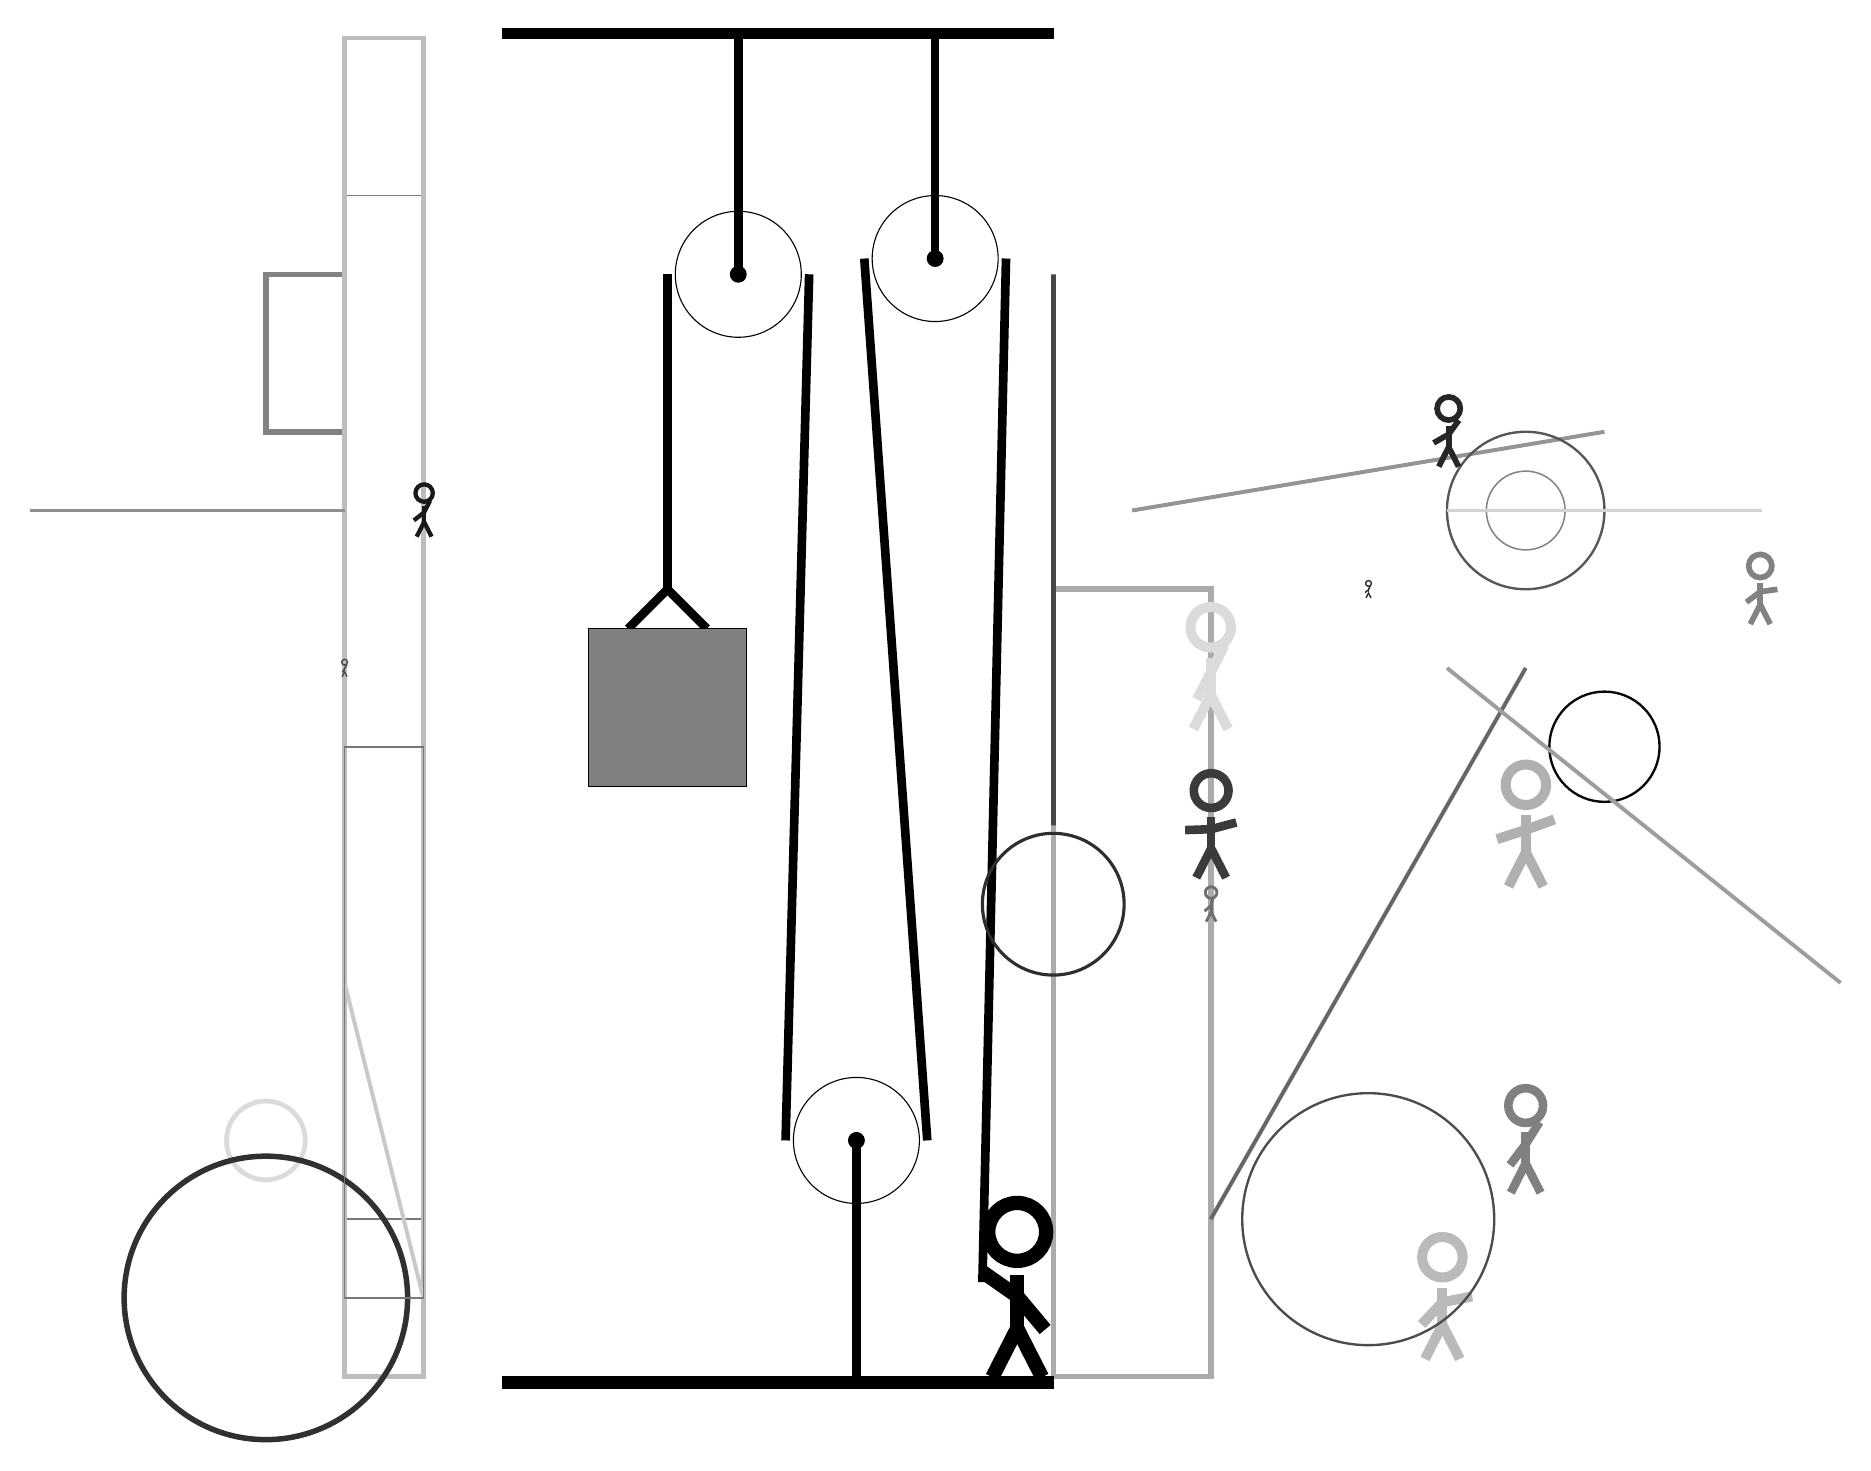
\begin{tikzpicture}
			%%%%% START %%%%%
			
			\draw[fill=black] (-2, 14) rectangle (5, 14.125);
			
			\draw (1, 11) circle (0.8);
			\draw[fill=black] (1, 11) circle (0.1);
			\draw[line width=1.1mm]  (1, 14) -- (1, 11);
			
			\draw[fill=white](2.5, 0) circle (0.8);
			\draw[fill=black] (2.5, 0) circle (0.1);
			\draw[line width=1.1mm]  (2.5, -3) -- (2.5, 0);
			
			\draw[fill=white](3.5, 11.2) circle (0.8);
			\draw[fill=black] (3.5, 11.2) circle (0.1);
			\draw[line width=1.1mm] (3.5, 14) -- (3.5, 11.2);
			
			\draw[line width=1.1mm] (-0.4, 6.5) -- (0.1, 7.0) -- (0.6, 6.5);
			\draw[fill=black!50] (-0.9, 6.5) rectangle (1.1, 4.5);
			
			\draw[line width=1.1mm] (0.1, 11) -- (0.1, 7.0);
			\centerarc[line width=1.1mm](1, 11)(0:180:0.9);
			\draw[line width=1.1mm](1.9, 11) -- (1.6, 0);
			\centerarc[line width=1.1mm](2.5, 0)(180:360:0.9);
			\draw[line width=1.1mm](3.4, 0) -- (2.6, 11.2);
			\centerarc[line width=1.1mm](3.5, 11.2)(0:180:0.9);
			\draw[line width=1.1mm](4.4, 11.2) -- (4.1, -1.8);
			
			\node[line width=0.4mm, color=black!50] at (11, 0) {\Strichmaxerl[6][53][58]};
			
			\draw[line width=0.2mm, color=black!53] (-4, -1) rectangle (-3, 12);
			\draw [line width=0.3mm, color=black!97](12, 5) circle (0.7);
			\draw[line width=0.7mm, color=black!49] (-4, 11) rectangle (-5, 9);
			\draw [line width=0.2mm, color=black!48](11, 8) circle (0.5);
			
			\draw[line width=0.7mm, color=black!33] (7, -3) rectangle (5, 7);
			\node[line width=0.7mm, color=black!14] at (7, 6) {\Strichmaxerl[7][63][63]};
			\node[line width=0.5mm, color=black!77] at (7, 4) {\Strichmaxerl[6][2][15]};
			\draw [line width=0.6mm, color=black!14](-5, 0) circle (0.5);
			
			\draw[line width=0.6mm, color=black!26] (-3, 14) rectangle (-4, -3);
			
			\draw[line width=0.5mm, color=black!42](6, 8) -- (12, 9);
			\draw[line width=0.5mm, color=black!21](-4, 2) -- (-3, -2);
			\draw [line width=0.7mm, color=black!81](-5, -2) circle (1.8);
			\draw [line width=0.3mm, color=black!66](11, 8) circle (1.0);
			\draw[line width=0.5mm, color=black!17](10, 8) -- (14, 8);
			\draw[line width=0.5mm, color=black!60](7, -1) -- (11, 6);
			
			\draw[line width=0.5mm, color=black!38](10, 6) -- (15, 2);
			\draw[line width=0.6mm, color=black!72] (5, 11) rectangle (5, 4);
			\node[line width=0.2mm, color=black!81] at (9, 7) {\Strichmaxerl[1][37][66]};
			
			\node[line width=0.4mm, color=black!90] at (-3, 8) {\Strichmaxerl[3][38][63]};
			\node[line width=0.5mm, color=black!85] at (10, 9) {\Strichmaxerl[4][30][54]};
			
			\draw[line width=0.5mm, color=black!44](-4, 8) -- (-8, 8);
			\node[line width=0.6mm, color=black!57] at (7, 3) {\Strichmaxerl[2][41][76]};
			\node[line width=0.3mm, color=black!71] at (-4, 6) {\Strichmaxerl[1][59][57]};
			\draw[line width=0.2mm, color=black!53] (-3, -2) rectangle (-4, 5);
			
			\node[line width=0.3mm, color=black!49] at (14, 7) {\Strichmaxerl[4][37][8]};
			\draw [line width=0.4mm, color=black!82](5, 3) circle (0.9);
			\node[line width=0.3mm, color=black!27] at (10, -2) {\Strichmaxerl[7][47][11]};
			
			\draw [line width=0.3mm, color=black!70](9, -1) circle (1.6);
			\node[line width=0.6mm, color=black!31] at (11, 4) {\Strichmaxerl[7][18][20]};
			
			\node at (4.5, -1.9) {\Strichmaxerl[10][-35][-50]};
			
			\draw[fill=black] (-2, -3) rectangle (5, -3.15);
			
			%%%%% END %%%%%
		\end{tikzpicture}
	\end{figure}	
\end{document}